\let\negmedspace\undefined
\let\negthickspace\undefined
\documentclass[journal]{IEEEtran}
\usepackage[a5paper, margin=10mm, onecolumn]{geometry}
%\usepackage{lmodern} % Ensure lmodern is loaded for pdflatex
\usepackage{tfrupee} % Include tfrupee package

\setlength{\headheight}{1cm} % Set the height of the header box
\setlength{\headsep}{0mm}     % Set the distance between the header box and the top of the text
\usepackage{gvv-book}
\usepackage{gvv}
\usepackage{cite}
\usepackage{amsmath,amssymb,amsfonts,amsthm}
\usepackage{algorithmic}
\usepackage{graphicx}
\usepackage{textcomp}
\usepackage{xcolor}
\usepackage{txfonts}
\usepackage{listings}
\usepackage{enumitem}
\usepackage{mathtools}
\usepackage{gensymb}
\usepackage{comment}
\usepackage[breaklinks=true]{hyperref}
\usepackage{tkz-euclide} 
\usepackage{listings}
% \usepackage{gvv}                                        
\def\inputGnumericTable{}                                 
\usepackage[latin1]{inputenc}                                
\usepackage{color}                                            
\usepackage{array}                                            
\usepackage{longtable}                                       
\usepackage{calc}                                             
\usepackage{multirow}                                         
\usepackage{hhline}                                           
\usepackage{ifthen}                                           
\usepackage{lscape}
\usepackage{circuitikz}

\renewcommand{\thefigure}{\theenumi}
\renewcommand{\thetable}{\theenumi}
\setlength{\intextsep}{10pt} % Space between text and floats


\numberwithin{equation}{enumi}
\numberwithin{figure}{enumi}
\renewcommand{\thetable}{\theenumi}




% Marks the beginning of the document
\begin{document}
\bibliographystyle{IEEEtran}
\vspace{3cm}

\title{EE\\2010}
\author{EE24BTECH11063 - Y.Harsha Vardhan Reddy}
\maketitle

\bigskip

\renewcommand{\thefigure}{\theenumi}
\renewcommand{\thetable}{\theenumi}

\section*{Q.1-Q.25 carry one mark each}

    \begin{enumerate}
    \item Power is transferred from system A to system B by an HVDC link as shown in the figure $\ref{fig:1}$ . If the voltages $V_{AB}$ and $V_{CD}$ are as indicated in the figure, and $I > 0$, then:
    	\begin{figure}[!ht]
			\centering
			\scalebox{0.5}{ % Adjust the scaling factor as needed
\begin{circuitikz}
\tikzstyle{every node}=[font=\large]

\draw  (0,12.25) rectangle (3.75,16);
\draw  (11.25,16) rectangle (15,12.25);
\draw (3.75,15.25) to[L ] (6.5,15.25);
\draw (9,15.25) to[L ] (11.25,15.25);
\draw (6.5,15.25) to[R] (9,15.25);
\node at (4.25,15.25) [circ] {};
\node at (11,15.25) [circ] {};
\draw (6.75,13) to[short] (6.75,13);
\draw (3.75,12.75) to[short] (11.25,12.75);
\node at (4.25,12.75) [circ] {};
\node at (11,12.75) [circ] {};
\draw [short] (4,15.25) -- (4,15.25);
\draw [short] (4,15.25) -- (4.5,15.25)node[pos=0.5,above, fill=white]{A};
\draw [short] (11,15.25) -- (11.25,15.25)node[pos=0.35,above, fill=white]{C};
\draw [short] (4,12.75) .. controls (4.75,12.75) and (5,12.75) .. (6,12.75)node[pos=0.15,below, fill=white]{B};
\draw [short] (10.5,12.75) -- (11.25,12.75)node[pos=0.5,below, fill=white]{D};
\draw [->, >=Stealth] (8.5,15.25) -- (9.25,15.25)node[pos=0.5,below, fill=white]{I};
\draw [->, >=Stealth] (6,17) -- (9,17)node[pos=0.5,above, fill=white]{Power Flow};
\draw [->, >=Stealth] (4.25,13.25) -- (4.25,14.75)node[pos=0.5,right, fill=white]{$V_{AB}$};
\draw [->, >=Stealth] (11,13.25) -- (11,14.75)node[pos=0.5,left, fill=white]{$V_{CD}$};
\draw [ line width=0.6pt](1.75,13.5) to[D] (1.75,15.25);
\draw (13,15.5) to[D] (13,13.75);
\draw (12.5,14) to[short] (13,14.5);
\draw (1.25,15) to[short] (1.75,14.5);
\draw [short] (0.75,12.25) -- (2.75,12.25)node[pos=0.5,below, fill=white]{Rectifier};
\draw [short] (12.25,12.25) -- (14.25,12.25)node[pos=0.5,below, fill=white]{Inverter};
\draw (-1,15) to[short] (0,15);
\draw (-1,14) to[short] (0,14);
\draw (-1,13) to[short] (0,13);
\draw (15,15) to[short] (16,15);
\draw (15,13.75) to[short] (16.25,13.75);
\draw (15,12.75) to[short] (16.25,12.75);
\draw [short] (-2.75,14.75) -- (-2.75,14.75)node[pos=0.5,below, fill=white]{AC};
\draw [short] (-2.75,13) -- (-2.75,13)node[pos=0.3,above, fill=white]{System A};
\draw [short] (17.75,13) -- (17.75,13)node[pos=0.5,above, fill=white]{System B};
\draw [short] (17.75,14.75) -- (17.75,14.75)node[pos=0.5,below, fill=white]{AC};
\end{circuitikz}
}
			\caption{}
			\label{fig:1}
	\end{figure}
    \begin{enumerate}
        \item $V_{AB} < 0, V_{CD} < 0, V_{AB} > V_{CD}$
        \item $V_{AB} > 0, V_{CD} > 0, V_{AB} < V_{CD}$
        \item $V_{AB} > 0, V_{CD} > 0, V_{AB} > V_{CD}$
        \item $V_{AB} > 0, V_{CD} < 0$
    \end{enumerate}

    \item A balanced three-phase voltage is applied to a star-connected induction motor, the phase to neutral voltage being $V$. The stator resistance, rotor resistance referred to the stator, stator leakage reactance, rotor leakage reactance referred to the stator, and the magnetizing reactance are denoted by $r_s$, $r_r'$, $x_s$, $x_r'$ and $X_m$, respectively. The magnitude of the starting current of the motor is given by:
    \begin{enumerate}
        \item $\frac{V}{\sqrt{(r_s + r_r')^2 + (x_s + x_r')^2}}$
        \item $\frac{V}{\sqrt{r_s^2 + (x_s + X_m)^2}}$
        \item $\frac{V}{\sqrt{(r_s + r_r')^2 + (X_m + x_s)^2}}$
        \item $\frac{V}{\sqrt{r_s^2 + (X_m + x_r')^2}}$
    \end{enumerate}

    \item Consider a step voltage wave of magnitude 1 pu traveling along a lossless transmission line that terminates in a reactor. The voltage magnitude across the reactor at the instant the traveling wave reaches the reactor is:
    \begin{figure}[!ht]
			\centering
			

\begin{circuitikz}
\tikzstyle{every node}=[font=\LARGE]
\draw (6.25,10.25) to[short] (6.25,10.25);
\draw (7.5,10.5) to[short] (3.75,10.5);
\draw (3.75,11.25) to[short] (4.5,11.25);
\draw (4.5,11.25) to[short] (4.5,10.5);
\draw [->, >=Stealth] (4.75,11) -- (5.25,11);
\draw (7.5,10.5) to[L,l={ \normalsize Reactor} ] (7.5,8.5);
\draw (7.5,8.5) to (7.5,8.25) node[ground]{};
\end{circuitikz}

			\caption{}
			\label{fig:2}
	\end{figure}

    \begin{enumerate}
	\begin{multicols}{4}
        \item $1$ pu
        \item $1$ pu
        \item $2$ pu
        \item $3$ pu
        \end{multicols}
    \end{enumerate}

    \item Consider two buses connected by an impedance of $(0 + j5) \Omega$. The bus 1 voltage is $100 \angle 30^\circ \, V$ and bus 2 voltage is $100 \angle 0^\circ \, V$. The real and reactive power supplied by bus 1, respectively, are:
    \begin{enumerate}
    \begin{multicols}{2}
        \item 1000 W, 268 VAr
        \columnbreak
        \item $-1000$ W, $-134$ VAr
        \end{multicols}
        \begin{multicols}{2}
        \item 276.9 W, $-56.7$ VAr
        \item $-276.9$ W, 56.7 VAr
        \end{multicols}
    \end{enumerate}

    \item A three-phase, 33 kV oil circuit breaker is rated 1200 A, 2000 MVA, 3 s. The symmetrical breaking current is:
    \begin{enumerate}
    \begin{multicols}{4}
        \item 1200 A
        \item 3600 A
        \item 35 kA
        \item 104.8 kA
        \end{multicols}
    \end{enumerate}

    \item Consider a stator winding of an alternator with an internal high-resistance ground fault. The currents under the fault condition are as shown in the figure. The winding is protected using a differential current scheme with current transformers of ratio 400/5 A as shown in figure$\ref{fig:3}$. The current through the operating coil is:
    \begin{figure}[!ht]
			\centering
			\scalebox{0.5}{
\begin{circuitikz}
\tikzstyle{every node}=[font=\large]

\draw [short] (-3.75,9) -- (16.25,9)node[pos=0.5,below, fill=white]{Operating coil};
\draw (-1.25,11) to[short] (13.75,11);
\draw (-3.75,14.75) to[short] (-3.75,9);
\draw (16.25,14.75) to[short] (16.25,9);
\draw (-3.75,14.75) to[L ] (-1.25,14.75);
\draw (13.75,14.75) to[L ] (16.25,14.75);
\draw (-1.25,11) to[short] (-1.25,14.75);
\draw (13.75,11) to[short] (13.75,14.75);
\draw (6,11) to[L ] (6,9);
\draw (1.25,14.75) to[L ] (11.25,14.75);
\draw (4.75,14.75) to[L ] (5.75,14.75);
\draw (7.5,14.75) to[L ] (8.5,14.75);
\draw (6.75,14.75) to[L ] (7.5,14.75);
\draw [short] (-5,14.75) -- (1.5,14.75)node[pos=0.05,above, fill=white]{CT ratio 400/5};
\draw [short] (12.75,14.75) -- (14.75,14.75);
\draw [short] (11,14.75) -- (17.5,14.75)node[pos=0.95,above, fill=white]{CT ratio 400/5};
\draw [->, >=Stealth] (12.75,14.75) -- (10.5,14.75)node[pos=0.5,below, fill=white]{(250 + j0) A};
\draw [->, >=Stealth] (2.25,14.75) -- (0,14.75)node[pos=0.5,below, fill=white]{(220 + j0) A};
\draw (6,13.25) to[european resistor] (8,13.25);
\draw (6,14.5) to[short] (6,13.25);
\draw (8,13.25) to (8,13) node[ground]{};
\end{circuitikz}
}
			\caption{}
			\label{fig:3}
	\end{figure}
    \begin{enumerate}
    \begin{multicols}{4}
        \item 0.1875 A
        \item 0.2 A
        \item 0.375 A
        \item 60 kA
	\end{multicols}
    \end{enumerate}
 \item   The zero-sequence circuit of the three-phase transformer shown in the figure$\ref{fig:4}$ is

\begin{figure}[!ht]
    
			\centering
			
\begin{circuitikz}
\tikzstyle{every node}=[font=\normalsize]
\draw [short] (4.5,10.25) .. controls (5.5,10.25) and (4.75,10.25) .. (7.75,10.25)node[pos=0,left, fill=white]{R};
\draw [short] (4.5,7.75) .. controls (5,7.75) and (4.25,7.75) .. (6.75,7.75)node[pos=0,left, fill=white]{Y};
\draw (7.75,8.75) to[L ] (8.75,7.75);
\draw (6.75,7.75) to[L ] (7.75,8.75);
\draw (7.75,8.75) to[L ] (7.75,10.25);
\draw (8.75,7.75) to[short] (8.75,7);
\draw [short] (4.5,7) .. controls (8,7) and (7.75,7) .. (8.75,7)node[pos=0,left, fill=white]{B};
\draw (11.5,7.5) to[L ] (11.5,10);
\draw (11.5,10) to[L ] (12.75,8.75);
\draw (11.5,7.5) to[L ] (12.75,8.75);
\draw [short] (14.75,8.75) .. controls (13.25,8.75) and (12.5,8.75) .. (13,8.75)node[pos=0,right, fill=white]{b};
\draw [short] (14.75,10) .. controls (11.75,10) and (12.5,10) .. (11.5,10)node[pos=0,right, fill=white]{r};
\draw [short] (14.75,7.5) .. controls (11.75,7.5) and (12.5,7.5) .. (11.5,7.5)node[pos=0,right, fill=white]{y};
\end{circuitikz}

			\caption{}
			\label{fig:4}
		\end{figure}
\begin{enumerate}

    \item[]

    \begin{figure}[H]
        \centering

        \begin{minipage}{0.45\linewidth}
            \centering
            \begin{circuitikz}
\tikzstyle{every node}=[font=\large]
\draw (5.75,10.5) to[L ] (7.75,10.5);
\draw (6.25,10.5) to[short, -o] (5.75,10.5) node[left] {R};
\draw (7.25,10.5) to[short, -o] (8,10.5) node[right] {r};
\draw [short] (5.75,9.25) -- (7.75,9.25)node[pos=0.55,below, fill=white]{G};
\end{circuitikz}
            \caption*{(a)}
        \end{minipage}%
        \hfill
        \begin{minipage}{0.45\linewidth}
            \centering
            \begin{circuitikz}
\tikzstyle{every node}=[font=\large]
\draw (5.75,10.5) to[L ] (7.75,10.5);
\draw (6.25,10.5) to[short, -o] (5.75,10.5) node[left] {R};
\draw (8.25,10.5) to[short, -o] (9,10.5) node[right] {r};
\draw [short] (5.75,9.25) -- (9,9.25)node[pos=0.55,below, fill=white]{G};
\end{circuitikz}
            \caption*{(b)}
        \end{minipage}

    \end{figure}

    \item[]

    \begin{figure}[H]
        \centering

        \begin{minipage}{0.45\linewidth}
            \centering
            \begin{circuitikz}
\tikzstyle{every node}=[font=\large]
\draw (5.75,10.5) to[L ] (7.75,10.5);
\draw (6.25,10.5) to[short, -o] (5.75,10.5) node[left] {R};
\draw (8.25,10.5) to[short, -o] (9,10.5) node[right] {r};
\draw [short] (5.75,9.25) -- (9,9.25)node[pos=0.55,below, fill=white]{G};
\draw (7.75,9.25) to[short] (7.75,10.5);
\end{circuitikz}
            \caption*{(c)}
        \end{minipage}%
        \hfill
        \begin{minipage}{0.45\linewidth}
            \centering
            \begin{circuitikz}
\tikzstyle{every node}=[font=\large]
\draw (6.75,10.5) to[L ] (8.75,10.5);
\draw (6.25,10.5) to[short, -o] (5.75,10.5) node[left] {R};
\draw (8.25,10.5) to[short, -o] (9,10.5) node[right] {r};
\draw [short] (5.75,9.25) -- (9,9.25)node[pos=0.55,below, fill=white]{G};
\draw (6.75,9.25) to[short] (6.75,10.5);
\end{circuitikz}
            \caption*{(d)}
        \end{minipage}

    \end{figure}
    
\end{enumerate}

\item Given that the op-amp is ideal, the output voltage $V_0$ is
	\begin{figure}[H]
    
			\centering
			
\begin{circuitikz}
\tikzstyle{every node}=[font=\normalsize]
\draw (5.75,11.25) to[short] (5.75,11.25);
\draw (7.5,5.5) to[battery1,l=$+2 V$] (7.5,6.75);
\draw (4.75,7.75) to[european resistor,l={ \normalsize R}] (7.5,7.75);
\draw (7.25,9.25) to[european resistor,l={ \normalsize 2R}] (10.25,9.25);
\draw [ fill={rgb,255:red,252; green,252; blue,252} ](9,7.25) node[op amp,scale=1, yscale=-1 ] (opamp2) {};
\draw [ fill={rgb,255:red,252; green,252; blue,252} ](opamp2.+) to[short] (7.5,7.75);
\draw [ fill={rgb,255:red,252; green,252; blue,252} ] (opamp2.-) to[short] (7.5,6.75);
\draw [ fill={rgb,255:red,252; green,252; blue,252} ](10.2,7.25) to[short](10.5,7.25);
\draw [short] (8.75,6.75) -- (8.75,6)node[pos=0.95,right, fill=white]{-10 V};
\draw [short] (8.75,7.75) -- (8.75,8.5)node[pos=0.85,right, fill=white]{+10 V};
\draw [short] (10,7.25) -- (11,7.25)node[pos=1,right, fill=white]{$V_0$};
\draw (7.25,7.75) to[short] (7.25,9.25);
\draw (10.25,9.25) to[short] (10.25,7.25);
\draw (7.5,5.5) to (7.5,5.25) node[ground]{};
\draw (4.75,7.75) to (4.75,7.5) node[ground]{};
\end{circuitikz}

			\caption{}
			\label{fig:5}
		\end{figure}

\begin{enumerate}
\begin{multicols}{4}
    \item  4 V
    \item  6 V
    \item  7.5 V
    \item  12.12 V
    \end{multicols}
\end{enumerate}

\item Assuming that the diodes in the given circuit shown in figure$\ref{fig:6}$ are ideal, the voltage $V_0$ is
\begin{figure}[H]
    
			\centering
			
\begin{circuitikz}
\tikzstyle{every node}=[font=\normalsize]
\draw (5.75,11.25) to[short] (5.75,11.25);
\draw (4,8.25) to[D] (6,8.25);
\draw (6,8.25) to[european resistor,l={ \normalsize 10k$\Omega$}] (8,8.25);
\draw (6,8.25) to[european resistor,l={ \normalsize 10k$\Omega$}] (6,6.75);
\draw (6,6.75) to[european resistor,l={ \normalsize 10k$\Omega$}] (6,5);
\draw [short] (6.5,6.75) .. controls (6.25,6.75) and (6.25,6.75) .. (6,6.75)node[pos=0,right, fill=white]{$V_0$};
\draw (9.25,8.25) to[D] (8,8.25);
\draw (4,8.25) to[battery1,l=$10V$] (4,5);
\draw (9.25,5) to[battery1,l=$15V$] (9.25,8.25);
\draw (4,5) to[short] (9.25,5);
\draw (6,5) to (6,4.75) node[ground]{};
\end{circuitikz}

			\caption{}
			\label{fig:6}
		\end{figure}

\begin{enumerate}
\begin{multicols}{4}
    \item  4 V
    \item  5 V
    \item  7.5 V
    \item  12.12 V
    \end{multicols}
\end{enumerate}

    \item The power electronic converter shown in the figure$\ref{fig:7}$ has a single-pole double-throw switch. The pole P of the switch is connected alternately to throws A and B. The converter shown is a:
    \begin{figure}[H]
    
			\centering
			
\begin{circuitikz}
\tikzstyle{every node}=[font=\normalsize]
\draw (5,12.25) to[battery ,l={ \normalsize $V_{in}$}] (5,14.75);
\draw (5,14.75) to[short, -o] (7,14.75) node[above] {$A$};
\draw (9.5,14.5) to[short, -o] (7.75,14.5) node[above] {$P$};
\draw (7.75,14.5) to[short] (7,14.5);
\draw (7,14.5) to[short] (7,15);
\draw (9.5,14.5) to[L ] (11.5,14.5);
\draw (11.5,14.5) to[R,l={ \normalsize $V_{out}$}] (11.5,12.75);
\draw (5,12.25) to[short] (11.5,12.25);
\draw (11.5,12.25) to[short] (11.5,13);
\draw (6,12.25) to[short, -o] (6,13.75) node[right] {$B$};
\end{circuitikz}

			\caption{}
			\label{fig:7}
		\end{figure}
    \begin{enumerate}
        \item step-down chopper (buck converter)
        \item half-wave rectifier
        \item step-up chopper (boost converter)
        \item full-wave rectifier
    \end{enumerate}

    \item Figure$\ref{fig:8}$ shows a composite switch consisting of a power transistor (BJT) in series with a diode. Assuming that the transistor switch and the diode are ideal, the I-V characteristic of the composite switch is:
    \begin{figure}[H]
    
			\centering
			
\begin{circuitikz}
\tikzstyle{every node}=[font=\LARGE]
\draw (8.75,11) to[D] (10.25,11);
\draw (10,11) to[short, -o] (10.75,11) node[above] {-};
\draw [->, >=Stealth] (8.25,11) .. controls (8.75,11) and (8.75,11) .. (9,11) node[pos=0.5,above, fill=white]{V};
\draw [short] (8,11) -- (9.25,11)node[pos=0.5,below, fill=white]{I};
\draw (8.25,11) to[Tnpn, transistors/scale=1.19] (6.25,11);
\draw (6.5,11) to[short, -o] (5.75,11) node[above] {+};
\end{circuitikz}

			\caption{}
			\label{fig:8}
		\end{figure}
    


\begin{enumerate}

    \item[]

    \begin{figure}[H]
        \centering

        \begin{minipage}{0.45\linewidth}
            \centering
            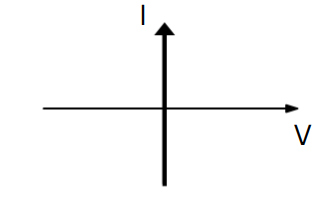
\includegraphics[width=\linewidth]{figs/24_options/a1.png}
            \caption*{(a)}
        \end{minipage}%
        \hfill
        \begin{minipage}{0.45\linewidth}
            \centering
            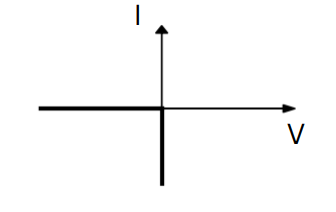
\includegraphics[width=\linewidth]{figs/24_options/a2.png}
            \caption*{(b)}
        \end{minipage}

    \end{figure}

    \item[]

    \begin{figure}[H]
        \centering

        \begin{minipage}{0.45\linewidth}
            \centering
            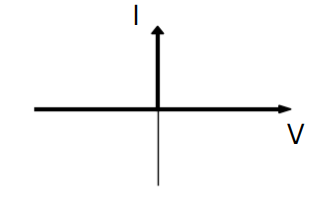
\includegraphics[width=\linewidth]{figs/24_options/a3.png}
            \caption*{(c)}
        \end{minipage}%
        \hfill
        \begin{minipage}{0.45\linewidth}
            \centering
            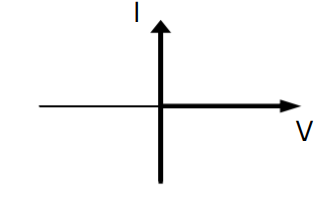
\includegraphics[width=\linewidth]{figs/24_options/a4.png}
            \caption*{(d)}
        \end{minipage}

    \end{figure}
    
\end{enumerate}
    \item The fully controlled thyristor converter in the figure$\ref{fig:9}$ is fed from a single-phase source. When the firing angle is $0^\circ$, the dc output voltage of the converter is 300 V. What will be the output voltage for a firing angle of $60^\circ$, assuming continuous conduction?
    \begin{figure}[H]
    
			\centering
			
\begin{circuitikz}
\tikzstyle{every node}=[font=\LARGE]
\draw (4.75,9.25) to[empty Zener diode] (4.75,10.75);
\draw (6.5,10.5) to[empty Zener diode] (6.5,12.25);
\draw (6.5,9.25) to[empty Zener diode] (6.5,10.5);
\draw (4.75,10.75) to[empty Zener diode] (4.75,12.25);
\draw (3.75,10.5) to[short] (6.5,10.5);
\draw (4.75,9.25) to[short] (8.5,9.25);
\draw (4.75,12.25) to[short] (6.75,12.25);
\draw (4.25,11) to[short] (4.75,11);
\draw (6.5,12.25) to[L ] (8.5,12.25);
\draw [short] (8.5,11.5) -- (8.5,12.25)node[pos=0.55,right, fill=white]{   +};
\draw (8.5,11.75) to[R,l={ \LARGE $V_{dc}$}] (8.5,10);
\draw [short] (8.5,10.25) -- (8.5,9.25)node[pos=0.5,right, fill=white]{   -};
\end{circuitikz}


			\caption{}
			\label{fig:9}
		\end{figure}
    \begin{enumerate}
    \begin{multicols}{4}
        \item 150 V
        \item 210 V
        \item 300 V
        \item $100\pi$ V
        \end{multicols}
    \end{enumerate}

    \item At $t = 0$, the function $f(t) = \frac{\sin t}{t}$ has:
    \begin{enumerate}
        \item a minimum
        \item a discontinuity
        \item a point of inflection
        \item a maximum
    \end{enumerate}

\end{enumerate}


\end{document}

